%!TEX root = ../main/main.tex
\section{METODOLOGIA}
%Guilherme você misturou a metodologia com a discussão de resultados. sugiro separar na metodologia vem a receita ingredientes - >dados de onde vem e qual a moldura limitação e os processos =métodos que serão utilizados porque e o que se espera como resultados ao utilizar. A discussão é o que você fez no Cap 4. só tomar cuidado com redundância

Explicar a qualidade de cursos superiores compreende uma tarefa complexa que pode ser objeto de várias abordagens e modelagens matemáticas distintas. 
Verificou-se na literatura relacionada ao tema trabalhado -- e em especial no trabalho de \citeonline{Coelho_2016}, que a análise sobre a qualidade do Enade como indicador se dá pela aplicação da técnica de Análise Envoltória de dados (\textit{Data Envelopment Analysis} - DEA), que se destina a encontrar as melhores práticas em uma amostra de organizações pertencentes a um conjunto de unidades comparáveis (\textit{Decision Making Units} - DMU).

Em resumo, esta técnica baseia-se na identificação de variáveis de entrada (\textit{input}) e saída (\textit{output}) que implicam na eficiência das unidades de decisão. As inferências são realizadas de modo a se determinar a proporção de diminuição (ou aumento) de uma determinada variável de entrada (ou saída) a fim de tornar uma DMU eficiente.

\subsection{Classificação da Pesquisa}
A presente pesquisa é qualitativa uma vez que almeja fornecer um entendimento objetivo sobre a metodologia de avaliação de cursos pelo INEP por intermédio da interpretação das narrativas dos autores utilizados como fundamentação. Por outro lado, este trabalho é também quantitativo, uma vez que a motivação principal é entender os indicadores por meio de informações numéricas. Portanto a investigação  qualitativa é complementada com a técnica de \textit{mineração dos dados} do censo dos cursos superiores, aliada ao uso de metodologia estatística sobre os mesmos.

\subsection{Ferramenta e Técnicas de análise de dados}
Para manipulação dos dados foi utilizado R. Trata-se de uma linguagem e um ambiente para computação estatística e criação de gráficos similar a linguagem \textit{S} desenvolvida pelo \textit{Bell Labs}. É uma aplicação livre e de código aberto sob a licença GNU/GPL \textit{(General Public License)} composta por uma extensa variedade de pacotes utilizados para as mais diferentes finalidades. O R é mantido por uma comunidade global de desenvolvedores e possui uma expressiva aceitação em pesquisas.

A crescente utilização deste ambiente de programação em substituição a outras soluções comerciais como \textit{Microsoft Excel}, \textit{IBM SPSS}, \textit{Sata} e \textit{Minitab} se deve a sua facilidade de uso e a possibilidade de aplicação em diversas áreas relacionadas à análise de dados. A opção por este ambiente se justifica pelo fato de o mesmo ser uma ferramenta gratuita e conter todos os recursos necessários às fases que compõem a aplicação da metodologia deste trabalho.

%\subsection{Técnicas de análise de dados}
Esta pesquisa utilizou um conjunto de três técnicas estatísticas destinadas à preparação e análise de dados. São elas: Análise Exploratória de Dados (AED), Análise do Componente Principal (ACP) e Análise Fatorial. Uma breve descrição relativa a cada uma delas será apresentada nas subseções a seguir.

%!TEX root = ../main/main.tex
\subsection{Análise Exploratória de dados}
	A análise exploratória neste trabalho foi possível pela versatilidade do pacote \lstinline{dplyr}\footnotemark. De acordo com \citeonline{dplyr} o pacote disponibiliza um conjunto extenso de instruções baseadas em ``verbos'' para manipulação do conjunto de dados. A ferramenta é uma iteração do pacote \lstinline{plyr} idealizada para lidar com \lstinline{dataframes}, por isso o prefixo \textit{d}.
	\footnotetext{De acordo com os autores, o \lstinline{plyr} tem três principais objetivos: identificar os verbos mais importantes para manipulação de dados e torná-los fáceis de utilizar com o R; promover rapidez para o tratamento dos dados em memória pela utilização do C++ como linguagem de desenvolvimento de componentes chaves do pacote; e utilizar a mesma interface para manipulação dos dados independentemente da forma como os mesmos estejam armazenados (seja como \lstinline{dataframe}, \textit{data tabel} ou \textit{database}).}

	Os dados utilizados estão disponíveis publicamente em formato \textit{Microsoft Excel (.xlsx)} e podem ser obtidos  diretamente do site do INEP. A presente análise utiliza dados referentes ao senso de 2015. A escolha deste ano se deu pelo fato de o ciclo de avaliação dos cursos superiores pelo INEP ser trienal. Desta forma, os dados mais atuais para utilização são relativos ao último ciclo avaliativo de 2015 no qual os cursos da Área de Ciências Sociais Aplicadas foram avaliados.

	Para elaboração da Análise Exploratória de Dados, procurou-se primeiramente descrever as variáveis presentes na base de dados do CPC, especificando nome, classe, além de uma breve definição. A seguir é apresentada a enumeração das mesmas juntamente aos seus atributos.

	\begin{enumerate}
	\item \textbf{Ano}: Categórica. Ano de realização do senso pelo INEP. Neste censo, foram avaliados os cursos em 2015.\
	\item \textbf{Código da IES}: Categórica. Código único de identificação das Instituições de ensino.\
	\item \textbf{Nome da IES}: Categórica. Nome da IES.\
	\item \textbf{Sigla da IES}: Categórica. Sigla da instituição de ensino.
	\item \textbf{Código do Curso}: Categórica. Código de identificação composto por números inteiros positivos, únicos para cada curso nacionalmente. Varia de 1 a 5001295.
	\item \textbf{Código da Área}: Categórica. Faz referência ao curso. Cada curso tem um código de área específico. Mesmos cursos em IES's distintas têm o mesmo código. Varia de 1 a 804.
	\item \textbf{Área de Enquadramento}: Categórica. Nome do curso superior.
	\item \textbf{Código do Município} Categórica. Código da cidade onde o curso é ofertado. Varia de 1100023 a 5300108. 756 níveis.
	\item \textbf{Município do Curso}: Categórica. Nome do município em que se localiza a IES que oferta o curso. 753 níveis.
	\item \textbf{Sigla da UF}: Categórica. Sigla do estado. 27 níveis.
	\item \textbf{Organização Acadêmica}: Categórica. As IES podem ter os possíveis 5 (cinco) níveis de enquadramento:
		\begin{enumerate}
			\item Centro Federal de Educação Tecnológica
			\item Centro Universitário 
			\item Faculdade 
			\item Instituto Federal de Educação, Ciência e Tecnologia 
			\item Universidade 
		\end{enumerate}
	\item \textbf{Categoria Administrativa}: enquadramento organizacional da IES em 10 (dez) níveis:
		\begin{enumerate}	
			\item Pessoa Jurídica de Direito Privado - Com fins lucrativos - Sociedade Civil                 
			\item Pessoa Jurídica de Direito Privado - Com fins lucrativos - Sociedade Mercantil ou Comercial
			\item Pessoa Jurídica de Direito Privado - Sem fins lucrativos - Associação de Utilidade Pública 
			\item Pessoa Jurídica de Direito Privado - Sem fins lucrativos - Fundação                       
			\item Pessoa Jurídica de Direito Privado - Sem fins lucrativos - Sociedade                       
			\item Pessoa Jurídica de Direito Público - Estadual                                              
			\item Pessoa Jurídica de Direito Público - Federal                                               
			\item Pessoa Jurídica de Direito Público - Municipal                                             
			\item Privada com fins lucrativos                                                                
			\item Privada sem fins lucrativos
		\end{enumerate}
	\item \textbf{Concluintes Inscritos}: Inteira, discreta. Número de estudantes inscritos para realizar a avaliação do Enade.\
	\item \textbf{Concluintes Participantes}: Inteira, discreta. Quantidade de estudantes que efetivamente realizaram a avaliação.\
	\item \textbf{Nota Bruta FG}: Real, contínua. Nota dos alunos na parte de formação geral em escala de 0 a 100.\
	\item \textbf{Nota Bruta - CE}: Real, contínua. Nota dos alunos na parte de conhecimento específico em escala de 0 a 100.
	\item \textbf{Nota Bruta - Geral}: Real, contínua. Média ponderada envolvendo as notas nas provas de conhecimentos específicos e gerais.
	\item \textbf{Nota Contínua do Enade}: Real, contínua. Nota atribuída com base no desempenho do estudante na prova do Enade, calculada para cada curso de graduação. Varia de 0 a 5.
	\item \textbf{Nota Bruta - Organização Didático-Pedagógica}: Real, contínua. Nota média dos alunos nas questões do questionário do estudante referentes à Organização Didático-Pedagógica em escala de 0 a 6.
	\item \textbf{Nota Padronizada - Organização Didático-Pedagógica}: Real, contínua. nota padronizada dos alunos nas questões do questionário do estudante referentes à Organização Didático-Pedagógica em escala de 0 a 6.
	\item \textbf{Nota Bruta - Infraestrutura e Instalações Físicas}: Real, contínua. Nota média dos alunos nas questões do questionário do estudante referentes à infraestrutura em escala de 0 a 6.
	\item \textbf{Nota Padronizada - Infraestrutura e Instalações Físicas}: Real, contínua. Nota padronizada dos alunos nas questões do questionário do estudante referentes à infraestrutura em escala de 0 a 6.
	\item \textbf{Nota Bruta - Oportunidades de Ampliação da Formação}: Real, contínua. Nota média dos alunos nas questões do questionário do estudante referentes à Oportunidades de ampliação em escala de 0 a 6.
	\item \textbf{Nota Padronizada - Oportunidades de Ampliação da Formação}: Real, contínua. nota padronizada dos alunos nas questões do questionário do estudante referentes à oportunidades de ampliação em escala de 0 a 6.
	\item \textbf{Concluintes Participantes com nota no Enem}: Inteira, discreta. Quantidade de estudantes que realizaram o Enem como forma de ingresso nas IES's.
	\item \textbf{Percentual de Concluintes participantes com nota no Enem}: Real, contínua. Relação entre os concluintes que participaram da avaliação do Enade e os que tiveram nota no Enem.
	\item \textbf{Nota Bruta - IDD}: Real, contínua. Indicador de diferença de desempenho. Mede o valor agregado pelo processo formativo ao desenvolvimento dos estudantes concluintes oferecido pelo curso. Mensura o valor agregado pelo curso  considerando resultado do Enade e as características dos estudantes ao ingressarem no curso avaliada pela nota do estudante no Enem. Nesta base de dados, variam de -23.6500 a 24.4700.
	\item \textbf{Nota Padronizada - IDD}: Real, contínua. Indicador de diferença de desempenho após padronização em escala de 0 a 5.
	\item \textbf{Nr. de Docentes}: Inteira, discreta. Quantidade de professores no curso.
	\item \textbf{Nota Bruta - Mestres}: Real, contínua. Percentual de mestres do curso de 0 a 100\%.
	\item \textbf{Nota Padronizada - Mestres}: Real, contínua. Nota padronizada atribuída ao percentual de mestres após padronização em escala de 0 a 5.
	\item \textbf{Nota Bruta - Doutores}: Real, contínua. Percentual de doutores do curso de 0 a 100\%.
	\item \textbf{Nota Padronizada - Doutores}: Real, contínua. Nota padronizada atribuída ao percentual de doutores após padronização em escala de 0 a 5.
	\item \textbf{Nota Bruta - Regime de Trabalho}: Real, contínua. Percentual de professores com regime integral + parcial do curso de 0 a 100\%.
	\item \textbf{Nota Padronizada - Regime de Trabalho}: Nota padronizada atribuída ao percentual de professores com regime integral + parcial após padronização.
	\item \textbf{CPC Contínuo}: Real, contínua. Conceito preliminar de curso é a nota atribuída ao curso superior, em escala de 0 a 5.
	\item \textbf{CPC Faixa}: Inteira, discreta. Variável resposta. Faixa do CPC em escala de 0 a 5.
	\end{enumerate}

	Quanto a estrutura da base de dados, e informações pertinentes ao censo algumas informações podem ser destacadas:

	\begin{enumerate}
	\item \textbf{Dimensões da base de dados}: 8121  linhas $\times$  38  colunas

	\item \textbf{Dados sobre o censo}:
		\begin{enumerate}
		\item Cursos avaliados:  8121
		\item IES's avaliadas:  1758
		\item Municípios com cursos avaliados:  753
		\item Estados com cursos avaliados:  27
		\item Percentual de participação nas provas:  81.4\%
		\end{enumerate}
	\item \textbf{Cursos por regiões}:
	% Please add the following required packages to your document preamble:
% \usepackage{booktabs}
% \usepackage{graphicx}
\begin{table}[H]
\centering
\resizebox{\textwidth}{!}{%
\begin{tabular}{@{}lllllll@{}}
\toprule
\textbf{Área de Enquadramento}           & \textbf{Centro Oeste} & \textbf{Nordeste} & \textbf{Norte} & \textbf{Sudeste} & \textbf{Sul} & \textbf{Total} \\ \midrule
ADMINISTRAÇÃO                            & 189                   & 312               & 97             & 841              & 367          & 1806           \\
DIREITO                                  & 117                   & 208               & 70             & 455              & 216          & 1066           \\
CIÊNCIAS CONTÁBEIS                       & 115                   & 190               & 71             & 444              & 224          & 1044           \\
TECNOLOGIA EM GESTÃO DE RECURSOS HUMANOS & 41                    & 69                & 17             & 314              & 82           & 523            \\
PSICOLOGIA                               & 39                    & 85                & 31             & 200              & 111          & 466            \\
PUBLICIDADE E PROPAGANDA                 & 30                    & 49                & 16             & 200              & 60           & 355            \\
TECNOLOGIA EM LOGÍSTICA                  & 15                    & 44                & 12             & 210              & 56           & 337            \\
JORNALISMO                               & 23                    & 49                & 22             & 126              & 55           & 275            \\
TECNOLOGIA EM MARKETING                  & 10                    & 37                & 7              & 167              & 50           & 271            \\
TECNOLOGIA EM GESTÃO FINANCEIRA          & 11                    & 23                & 5              & 139              & 45           & 223            \\
TECNOLOGIA EM PROCESSOS GERENCIAIS       & 9                     & 24                & 7              & 113              & 63           & 216            \\
CIÊNCIAS ECONÔMICAS                      & 15                    & 36                & 9              & 83               & 48           & 191            \\
DESIGN                                   & 8                     & 20                & 5              & 70               & 75           & 178            \\
TECNOLOGIA EM GESTÃO COMERCIAL           & 9                     & 32                & 6              & 77               & 46           & 170            \\
TURISMO                                  & 16                    & 35                & 10             & 61               & 27           & 149            \\
TECNOLOGIA EM GASTRONOMIA                & 10                    & 24                & 2              & 49               & 22           & 107            \\
RELAÇÕES INTERNACIONAIS                  & 9                     & 8                 & 5              & 58               & 21           & 101            \\
TEOLOGIA                                 & 8                     & 14                & 5              & 37               & 30           & 94             \\
TECNOLOGIA EM DESIGN DE INTERIORES       & 8                     & 14                & 2              & 38               & 20           & 82             \\
TECNOLOGIA EM GESTÃO DA QUALIDADE        & 6                     & 6                 & 48             & 15               & 6            & 81             \\
TECNOLOGIA EM COMÉRCIO EXTERIOR          & 2                     & 3                 & 2              & 57               & 16           & 80             \\
TECNOLOGIA EM DESIGN GRÁFICO             & 6                     & 12                & 4              & 43               & 12           & 77             \\
TECNOLOGIA EM GESTÃO PÚBLICA             & 15                    & 11                & 4              & 19               & 16           & 65             \\
SECRETARIADO EXECUTIVO                   & 7                     & 10                & 4              & 22               & 18           & 61             \\
TECNOLOGIA EM DESIGN DE MODA             & 2                     & 13                & 2              & 22               & 19           & 58             \\
ADMINISTRAÇÃO PÚBLICA                    & 6                     & 16                & 2              & 19               & 8            & 51             \\ \bottomrule
\end{tabular}%
}
\caption{Cursos por região}
\label{my-label}
\end{table}
	\pagebreak
	\item \textbf{Percentual de cursos por Organização Acadêmica}: 
	\begin{figure}[H]
		\centering
		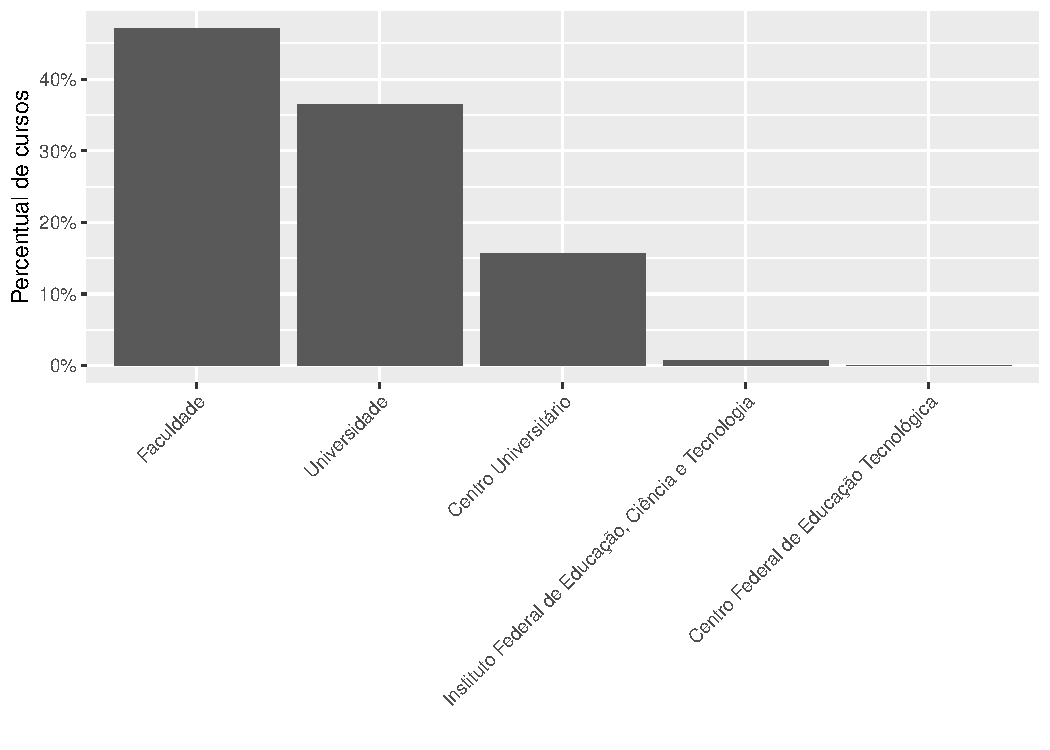
\includegraphics[scale=.90]{../../graficos/latex-graph-percent-de-cursos-p-org-acad.pdf}
		\caption{Percentual de cursos por organização acadêmica}
		\label{fig: graf-percent-cursos-org-acad}
	\end{figure}
	\pagebreak
	\item \textbf{Percentual de cursos por Categoria Administrativa}:
	\begin{figure}[H]
		\centering
		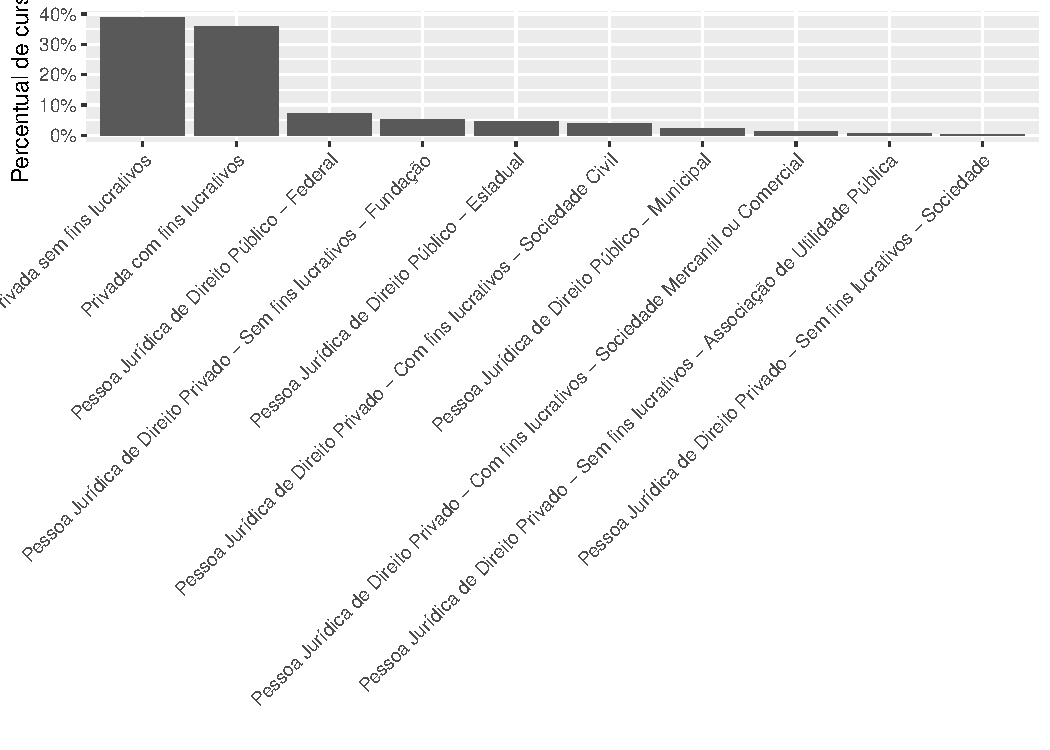
\includegraphics[scale=.9]{../../graficos/latex-graph-percent-de-cursos-p-cat-adm.pdf}
		\caption{Percentual de cursos por categoria administrativa}
		\label{fig: graf-percent-cursos-cat-adm}
	\end{figure}
	\item \textbf{IES por categoria administrativa}:
	% Please add the following required packages to your document preamble:
% \usepackage{booktabs}
% \usepackage{graphicx}
\begin{table}[H]
\centering
\resizebox{\textwidth}{!}{%
\begin{tabular}{@{}ll@{}}
\toprule
\textbf{Categoria Administrativa}                                                           & \textbf{Total} \\ \midrule
Privada com fins lucrativos                                                                 & 681            \\
Privada sem fins lucrativos                                                                 & 671            \\
Pessoa Jurídica de Direito Privado - Sem fins lucrativos - Fundação                         & 94             \\
Pessoa Jurídica de Direito Público - Federal                                                & 91             \\
Pessoa Jurídica de Direito Privado - Com fins lucrativos - Sociedade Civil                  & 70             \\
Pessoa Jurídica de Direito Público - Estadual                                               & 68             \\
Pessoa Jurídica de Direito Público - Municipal                                              & 43             \\
Pessoa Jurídica de Direito Privado - Com fins lucrativos - Sociedade Mercantil ou Comercial & 25             \\
Pessoa Jurídica de Direito Privado - Sem fins lucrativos - Associação de Utilidade Pública  & 9              \\
Pessoa Jurídica de Direito Privado - Sem fins lucrativos - Sociedade                        & 6              \\ \bottomrule
\end{tabular}%
}
\end{table}

	\item \textbf{Variável resposta}: Conceito Preliminar de Curso. Sobre a variável resposta \textit{CPC Faixa} foi observado que 12,97\% dos cursos não obtiveram notas\footnotemark. Os demais cursos estão relacionados na figura \ref{graf: cursos-com-conceito} e na tabela \ref{tbl: cursos-com-conceito}:
	\footnotetext{Cursos não reconhecidos: 847 (10.4\%);
	Cursos sem conceito: 205 (2.52\%);
	Cursos sub judice: 2 (0.0246\%)}

	\begin{figure}[H]
		\centering
		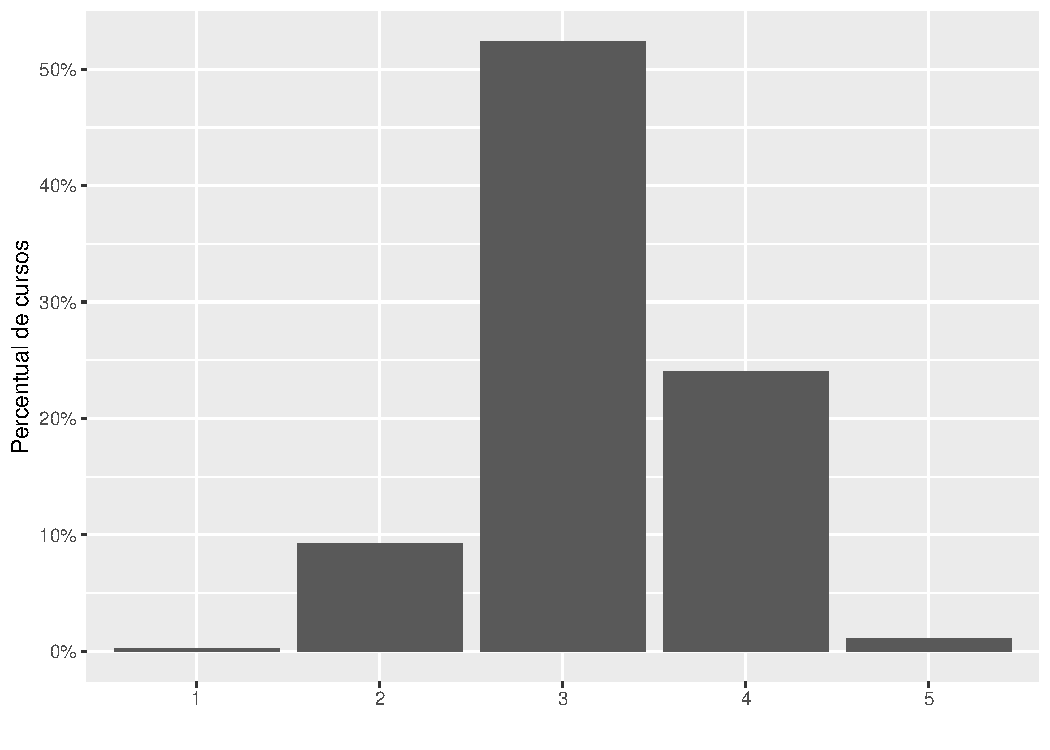
\includegraphics[scale=.75]{../../graficos/latex-graph-cursos-com-conceito.pdf}
		\caption{Cursos com conceito}
		\label{graf: cursos-com-conceito}
	\end{figure}

	% Please add the following required packages to your document preamble:
% \usepackage{booktabs}
\begin{table}[H]
\centering
\begin{tabular}{@{}lll@{}}
\toprule
\textbf{Conceito} & \textbf{Frequência} & \textbf{Percentual} \\ \midrule
1                 & 22                  & 0.3\%               \\
2                 & 753                 & 9.3\%               \\
3                 & 4252                & 52.4\%              \\
4                 & 1949                & 24.0\%              \\
5                 & 91                  & 1.1\%               \\ \bottomrule
\end{tabular}
\caption{Cursos com conceito}
\label{tbl: cursos-com-conceito}
\end{table}

	\item \textbf{Análise das variáveis numéricas}: Sabe-se que alguns cursos não obtiveram conceito pelo fato de estarem na condição de não reconhecidos, sem conceito ou sub judice. Foi observado, contudo que tais cursos apesar de estarem com o campo CPC Faixa vazios (e portanto sem a principal variável, a de resposta), tiveram notas nas variáveis preditoras. A partir desta constatação foi possível concluir que a utilização dessas observações nas modelagens estatísticas traria prejuízos significativos em termos de precisão.

	Com a finalidade de minimizar os efeitos da influência de observações vazias, duas abordagens foram inicialmente estudadas. A primeira consiste em utilizar o método de imputação de dados denominado $k$-NN\footnote{Este método encontra-se implementado no pacote \lstinline{DMwR} sob autoria de \citeonline{DMwR}.}~(\textit{k-Nearest Neighbors algorithm}) procura estimar o valor da observação vazia a partir de um parâmetro $k$ que representa a distância deste aos seus $k$ vizinhos mais próximos.

	Na segunda abordagem foram omitidas as observações vazias sob a hipótese de que as mesmas estão suficientemente representadas pelas demais observações. Desta forma a criação de um modelo não perderia eficiência nem estaria enviesado. A tabela \ref{tbl: sumario-estatisico-com-knn} contém a sumarização estatística das variáveis preditoras. Nela foi utilizada a técnica de estimação das observações vazias pelo método $k$-NN. Não foram verificadas diferenças significativas nas medidas estatísticas que implicassem em impossibilidade de estimação pelo método proposto.

	Como \citeonline[p.~2]{josse2016missmda} de forma bem elucidativa aborda, manipular bases com dados faltantes utilizando PCA pode ser uma tarefa complicada pela limitação que alguns softwares têm em gerar resultados a partir de campos vazios. Segundo esse autor a aplicação do método $k$-NN pressupõe que as variáveis estejam sob distribuição Gaussiana e é seguramente um método de imputação de variáveis contínuas bastante popular \Ibidem[p.~24]{josse2016missmda}. A sumarização estatística utilizando o método pode ser vista na tabela \ref{tbl: sumario-estatisico-com-knn}.

	% Please add the following required packages to your document preamble:
% \usepackage{booktabs}
% \usepackage{graphicx}
\begin{table}[H]
\centering
\resizebox{\textwidth}{!}{%
\begin{tabular}{@{}llllllll@{}}
\toprule
\textbf{Variável}                                         & \textbf{Média} & \textbf{Desvio padrão} & \textbf{Mediana} & \textbf{Moda} & \textbf{Mínimo} & \textbf{Máximo} & \textbf{n} \\ \midrule
Concluintes Inscritos                                     & 67.6625        & 204.194                & 39               & 25            & 1               & 11155           & 8121       \\
Concluintes Participantes                                 & 55.0494        & 162.6907               & 32               & 20            & 0               & 10059           & 8121       \\
Nota Bruta - FG                                           & 54.1955        & 6.2626                 & 53.8867          & 55.8          & 4.7127          & 80.65           & 8121       \\
Nota Bruta - CE                                           & 42.5299        & 8.228                  & 41.46            & 44.6          & 4.1746          & 80.8091         & 8121       \\
Nota Bruta - Geral                                        & 45.4587        & 7.0596                 & 44.7091          & 47.6          & 4.3141          & 79.75           & 8121       \\
Nota Contínua do Enade                                    & 2.3915         & 0.8577                 & 2.324            & 5             & 0               & 5               & 8121       \\
Nota Bruta - Organização Didático-Pedagógica              & 5.2105         & 0.481                  & 5.221            & 6             & 1.7121          & 6               & 8121       \\
Nota Padronizada - Organização Didático-Pedagógica        & 3.0204         & 1.1832                 & 3.0213           & 5             & 0               & 5               & 8121       \\
Nota Bruta - Infraestrutura e Instalações Físicas         & 4.9685         & 0.6723                 & 5.0136           & 6             & 2               & 6               & 8121       \\
Nota Padronizada - Infraestrutura e Instalações Físicas   & 3.1313         & 1.2076                 & 3.1954           & 5             & 0               & 5               & 8121       \\
Nota Bruta - Oportunidades de Ampliação da Formação       & 4.5659         & 0.8142                 & 4.5565           & 6             & 1.1905          & 6               & 8121       \\
Nota Padronizada - Oportunidades de Ampliação da Formação & 2.9541         & 1.1725                 & 2.9522           & 5             & 0               & 5               & 8121       \\
Concluintes Participantes com nota no Enem                & 28.7791        & 67.3562                & 17               & 7             & 1               & 3842            & 8121       \\
Percentual de Concluintes participantes com nota no Enem  & 0.5344         & 0.206                  & 0.5385           & 0.5           & 0.0143          & 1               & 8121       \\
Nota Bruta - IDD                                          & -0.1043        & 2.3789                 & -0.0948          & -1.5685       & -23.6519        & 24.4723         & 8121       \\
Nota Padronizada - IDD                                    & 2.4782         & 0.8428                 & 2.4758           & 0             & 0               & 5               & 8121       \\
Nr. de Docentes                                           & 26.1061        & 21.6867                & 20               & 16            & 0               & 298             & 8121       \\
Nota Bruta - Mestres                                      & 0.7633         & 0.2083                 & 0.8077           & 1             & 0               & 1               & 8121       \\
Nota Padronizada - Mestres                                & 3.5552         & 1.2234                 & 3.7796           & 5             & 0               & 5               & 8121       \\
Nota Bruta - Doutores                                     & 0.3124         & 0.2219                 & 0.2766           & 0             & 0               & 1               & 8121       \\
Nota Padronizada - Doutores                               & 1.7291         & 1.2051                 & 1.5541           & 0             & 0               & 5               & 8121       \\
Nota Bruta - Regime de Trabalho                           & 0.7592         & 0.238                  & 0.8125           & 1             & 0               & 1               & 8121       \\
Nota Padronizada - Regime de Trabalho                     & 3.6919         & 1.2766                 & 3.9688           & 5             & 0               & 5               & 8121       \\
CPC Contínuo                                              & 2.6111         & 0.5807                 & 2.609            & 1.0491        & 0.4257          & 4.6885          & 8121       \\
CPC Faixa                                                 & 3.1711         & 0.6371                 & 3                & 3             & 1               & 5               & 8121       \\ \bottomrule
\end{tabular}%
}
\caption{Sumarização da base de dados após uso do método $k$-NN: medidas estatísticas básicas}
\label{tbl: sumario-estatisico-com-knn}
\end{table}
	\end{enumerate}
\pagebreak


%!TEX root = ../main/main.tex
\subsection{Análise do Componente Principal}
\subsubsection{Padronização das variáveis}

De acordo com \citeonline[p.~98]{larose2015data} a padronização dos dados precede a aplicação da Análise do Componente Principal - ACP (ou \textit{Principal Component Analysis}). Isso fica evidente com base na observação da sumarização estatística apresentada na tabela \ref{tbl: sumario-estatisico-com-knn}. Nesta tabela é possível observar a desproporcionalidade dos desvios-padrão entre as variáveis. Concluintes Inscritos, por exemplo, tem um desvio 896 vezes maior que Nota Bruta - Regime de Trabalho. Ainda de acordo com o mesmo autor, a padronização tem como principal objetivo evitar que a influência de uma variável domine a da outra no espectro de variabilidade.

Tanto a ACP como a AF (Análise do Fator, como será visto adiante) fizeram amplo uso do pacote \lstinline{psych}\footnote{Possui ferramentas estatísticas de propósito geral para aplicações em psicometria, personalidade e psicologia experimental.}. Dada a sua importância, este pacote constitui elemento chave para a aplicação das metodologias estatísticas desta pesquisa. De acordo com \citeonline{psych}, abarca um conjunto de funções para análise multivariada permitindo a criação de estatísticas descritivas. Dentre estas funções podem ser destacadas \lstinline{fa} e \lstinline{principal} que possibilitaram a computação dos carregamentos para a AF e ACP, respectivamente.

A padronização dos dados foi feita com a utilização da função \lstinline{scales} contida na instalação básica do R. Esta função posiciona as variáveis contínuas em uma unidade de escala pela subtração de sua média e divisão pelo desvio padrão (procedimento denominado \textit{z-scoring}). Isso torna o desvio padrão das mesmas 1 e a média 0. Em termos matemáticos a padronização pode ser expressa pela seguinte equação: 

\begin{equation}
Z_{i}=\dfrac{X_{i}-\mu_{i}}{\sigma_{ii}}
\end{equation}

Foi observado que o \textit{dataset} do CPC contém, para cada nota bruta, uma nota padronizada. Além disso, segundo \citeonline{INEP_2017} a metodologia utilizada para produção destas notas é expressa pela seguinte equação: 

\begin{equation}
Z_{FGj}=\dfrac{FG_{kj}-\overline{FG}_k}{S_{FGk}}
\end{equation}


Onde,

\begin{itemize}[label={}]
\item $Z_{FGj}$ é o afastamento padronizado em $FG$ da unidade de observação $j$;
\item $FG_{kj}$ é a nota bruta em $FG$ da $j$-ésima unidade de observação da área de avaliação $k$;
\item $\overline{FG}_k$ é a média em $FG$ da área de avaliação $k$; e
\item $S_{FGk}$ é o desvio-padrão em $FG$ da área de avaliação $k$.
\end{itemize}

Nesta pesquisa optou-se por manter tais variáveis no conjunto de preditoras. Esta decisão foi tomada com base na verificação de que tal metodologia é aplicada para a composição da respectiva variável. Além do mais, a mesma não necessariamente implica em desvio padrão unitário e média 0 quando a análise é feita sobre a totalidade de observações, como pode ser observado na tabela \ref{tbl: vars-padronizadas-inep}. 

% Please add the following required packages to your document preamble:
% \usepackage{booktabs}
% \usepackage{graphicx}
\begin{table}[H]
\centering
\resizebox{\textwidth}{!}{%
\begin{tabular}{@{}llllllll@{}}
\toprule
\textbf{Variáveis padronizadas pelo INEP}                 & \textbf{Média} & \textbf{Desvio pradrão} & \textbf{Mediana} & \textbf{Moda} & \textbf{Mínimo} & \textbf{Máximo} & \textbf{n} \\ \midrule
Nota Padronizada - Organização Didático-Pedagógica        & 3.0202         & 1.1832                  & 3.0212           & 5             & 0               & 5               & 8121       \\
Nota Padronizada - Infraestrutura e Instalações Físicas   & 3.1312         & 1.2076                  & 3.1951           & 5             & 0               & 5               & 8121       \\
Nota Padronizada - Oportunidades de Ampliação da Formação & 2.9541         & 1.1724                  & 2.9519           & 5             & 0               & 5               & 8121       \\
Nota Padronizada - IDD                                    & 2.4801         & 0.8406                  & 2.4773           & 0             & 0               & 5               & 8121       \\
Nota Padronizada - Mestres                                & 3.5556         & 1.2232                  & 3.7834           & 5             & 0               & 5               & 8121       \\
Nota Padronizada - Doutores                               & 1.7295         & 1.2049                  & 1.5556           & 0             & 0               & 5               & 8121       \\
Nota Padronizada - Regime de Trabalho                     & 3.6922         & 1.2768                  & 3.9688           & 5             & 0               & 5               & 8121       \\ \bottomrule
\end{tabular}%
}
\caption{Estatísticas sobre as variáveis padronizadas pelo INEP}
\label{tbl: vars-padronizadas-inep}
\end{table}

\subsubsection{Matriz de correlação das variáveis preditoras}

De acordo com \citeonline[p.~98]{larose2015data} a próxima etapa na Análise do Componente Principal consiste em verificar a existência de correlações entre as 23 variáveis preditoras e, portanto, a ocorrência de multicolinearidade. Duas variáveis do dataset são de resposta: CPCC refere-se à nota contínua do CPC e CPCF é a nota escalonada. Desta forma temos um total de 25 variáveis (23 preditoras e 2 de resposta).

A dificuldade em fazer uma matriz de correlação com as variáveis do CPC está em determinar quais das 25 variáveis apresentam correlação umas com as outras. A quantidade de variáveis preditoras é considerável e não é possível afirmar que as mesmas não apresentam correlação mútua.

Segundo \citeonline[p.~92]{larose2015data}, modelar uma relação utilizando um número de variáveis muito grande pode complicar mais do que explicar e viola dois princípios básicos. O primeiro é o da parcimônia segundo o qual é preciso manter a quantidade de variáveis preditoras em uma quantidade mínima de forma que haja facilidade na interpretação. O segundo é a tendência ao \textit{overfittig} que diz que a generalidade dos resultados pode dificultar a formação de novos resultados com a mudança dos dados de entrada.

Para análise de correlação foi utilizada a matriz correlograma\footnotemark~da figura \ref{fig: matriz-correlograma1}. Nesta matriz as variáveis são dispostas de forma que é possível determinar para cada uma o seu nível de correlação com os seus pares. Isso possibilita a verificação de possíveis ocorrências de multicolinearidade.
\footnotetext{Esta matriz é criada por intermédio da função \lstinline{corrplot} do pacote de mesmo nome. De acordo com seus criadores, \citeonline{corrplot2017}, o pacote permite visualizar matrizes de correlação e intervalos de confiança. Também contém algoritmos para reordenação de matrizes.}

\begin{figure}[H]
		\centering
		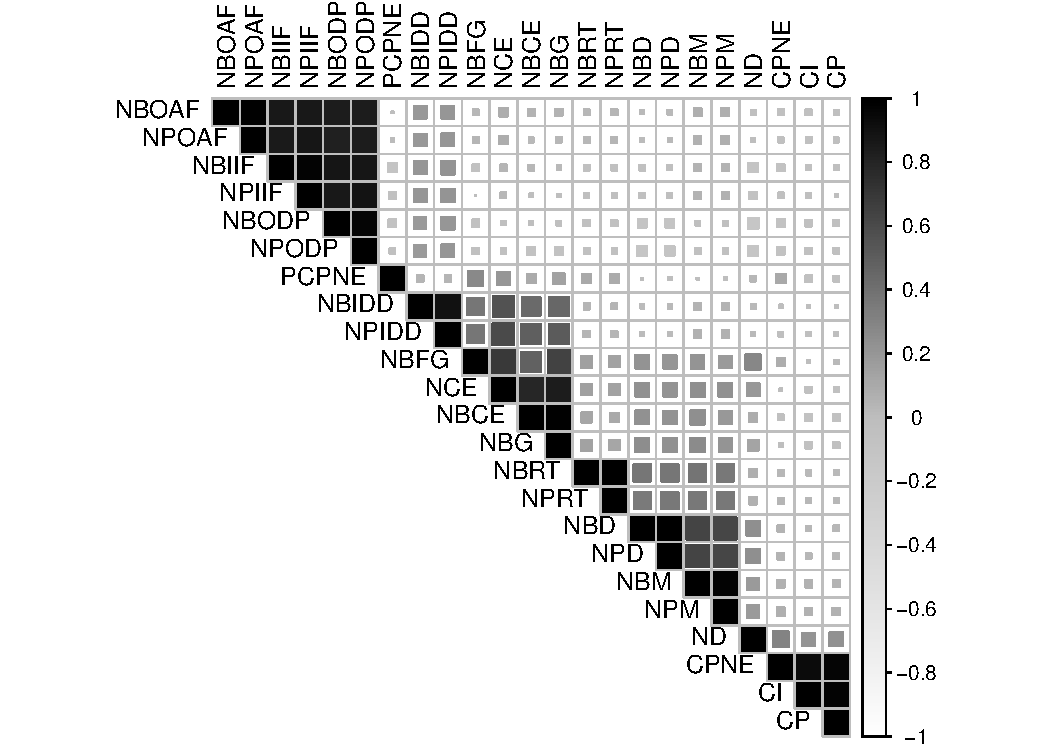
\includegraphics[scale=.75]{../../graficos/latex-graph-matriz-correlacao}
		\caption{Matriz correlograma: correlação entre os pares de variáveis segundo uma escala de cor.}
		\label{fig: matriz-correlograma1}
\end{figure}

Nesta matriz, a ordenação das variáveis foi feita por hierarquia de correlação, ou seja, da esquerda para direita, iniciando pelas correlações mais fortes. Com base na observação nas intensidades das cores, podemos verificar alguns trechos de correlações consideráveis especialmente nas variáveis relacionadas às oportunidades de ampliação da formação e infra-estrutura e instalações físicas.

Na figura \ref{fig: matriz-correlograma-2-bandas} vemos a representação das duas bandas da matriz correlograma. As variáveis assumem ordenamento de acordo com o índice de correlação e são posteriormente agrupadas em \textit{clusters}.

\begin{figure}[H]
		\centering
		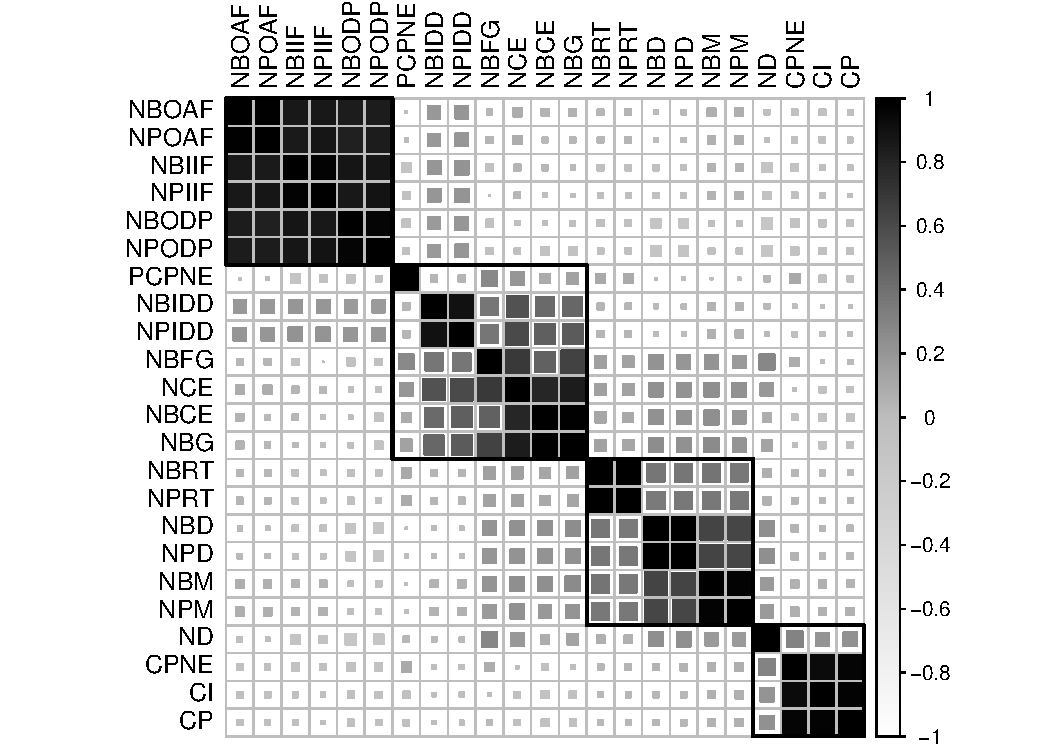
\includegraphics[scale=.75]{../../graficos/latex-graph-matriz-correlacao2.pdf}
		\caption{Matriz correlograma com as duas bandas}
		\label{fig: matriz-correlograma-2-bandas}
\end{figure}

Uma visualização alternativa das correlações pode ser obtida por meio da função \lstinline{shinypairs} do pacote \lstinline{pairsD3}. Este pacote 
permite produzir uma matriz interativa de gráficos de dispersão \cite{pairsD3}. É possível selecionar interativamente, de forma gradual dentre as variáveis preditoras, as que formarão a matriz de correlações. Com base nessa seleção de variáveis, copia-se da tela do \lstinline{shiny}\footnote{Facilitador de visualização interativa de dados. Para maiores informações visitar \url{https://shiny.rstudio.com}} o código que permite replicar a matriz com a função \lstinline{pairs}. 

Na figura \ref{fig: scatter-plot} podemos ver a formação do \textit{scatter-plot} com combinações\footnotemark~ de variáveis obtidas pela interface do \lstinline{pairsD3}.
\footnotetext{É importante observar que, dada a alta quantidade de variáveis contidas na base de dados, não é possível afirmar que a configuração de variáveis mostrada na matriz da figura \ref{fig: scatter-plot} contém combinação de pares com maior correlação. Experimentações foram feitas com variações de pares tendo como referência a matriz correlograma da figura \ref{fig: matriz-correlograma-2-bandas}. Para representação com todas as 23 variáveis preditoras seria necessário espaço suficiente para alocar 529 relações, muito além das dimensões das páginas deste trabalho.}

\begin{figure}[H]
		\centering
		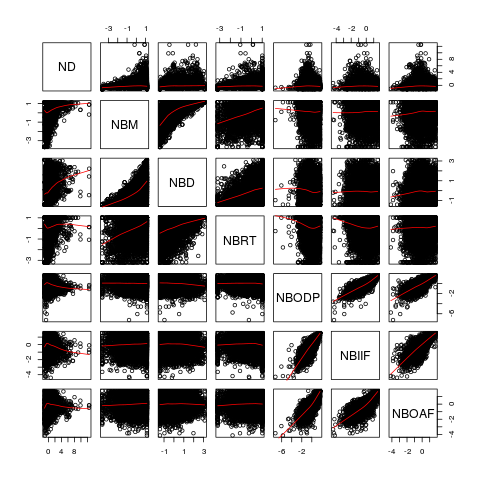
\includegraphics[scale=.80]{../../graficos/latex-graph-pairs.png}
		\caption{Matriz de pares de variáveis}
		\label{fig: scatter-plot}
\end{figure}

Devido ao elevado número de preditoras, esta forma de visualização, apesar de precisa, torna-se prejudicada. Contudo, o diagrama de matriz e a matriz de correlação são duas formas de olhar para a mesma coisa. \cite[p.~98]{larose2015data}

\subsubsection{Aplicação da Análise do Componente Principal}

De acordo com \citeonline[p.~98]{larose2015data} a ACP (Análise do Componente Principal) é a ferramenta mais adequada quando são analisadas variáveis em multicolinearidade. Isto é, tenta-se explicar a estrutura de correlações com base em combinações lineares, também chamadas de componentes. A variabilidade total de todas as variáveis pode ser contabilizada por um conjunto de componentes, uma vez que existe a mesma quantidade de informações nos mesmos em relação ao conjunto original.

Em outras palavras, a análise do componente principal procura reduzir a dimensão de um determinado conjunto de características pela criação de um novo conjunto de propriedades representativas devendo, para tanto, contabilizar a maior variância possível.

\subsubsection{Componentes Principais}

De acordo com \citeonline[p.~95--96]{larose2015data} a ACP é uma técnica de análise que se fundamenta em três corolários:

\begin{enumerate}
\item Assumindo que cada variável preditora possa ser representada em forma de vetor; que o conjunto dessas variáveis tenha sido padronizado e que a quantidade total de variáveis seja $m$, a variabilidade total do grupo de variáveis é igual a soma de cada vetor individual, que é igual à soma dos \textit{eigenvectors\footnotemark}, que é o total de variáveis preditoras. Desta forma, em termos matemáticos temos que:
\footnotetext{Em algebra linear, um \textit{eigenvector} ou vetor característico de uma transformação linear é um vetor não nulo que se altera somente por um fator escalar quando uma transformação linear é aplicada ao mesmo.}

\begin{equation}
\sum_{i=1}^m Var(Y_i) = \sum_{i=1}^m Var(Z_i) = \sum_{i=1}^m \lambda_i = m
\end{equation}

Onde,
\begin{itemize}[label={}]
\item $Y_i$ é o $i$-ésimo componente principal;
\item $Z_i$ é o $i$-ésimo vetor $Z$ (variável preditora pós padronização);
\item $\lambda_i$ é o $i$-ésimo \textit{eigenvector} da variável preditora.
\end{itemize}
\item A proporção de variabilidade total que explica o $i$-ésimo componente principal é a razão entre o $i$-ésimo \textit{eigenvector} pelo total de variáveis, isto é, $\dfrac{\lambda_i}{m}$.
\end{enumerate}

A listagem \ref{lst:loadings_pca} é o resultado da computação e visualização dos componentes principais das 23 preditoras sendo cada célula o peso de um componente:
\pagebreak
\begin{lstlisting}[label={lst:loadings_pca}, captionpos=b, caption={Computação dos carregamentos da Análise do Componente Principal}]
Loadings:
      PC1    PC2    PC3    PC4    PC5   
CI            0.103  0.639  0.722       
CP            0.108  0.642  0.734       
NBFG   0.175  0.624 -0.271  0.234       
NBCE   0.236  0.679 -0.440  0.195       
NBG    0.245  0.732 -0.445  0.223       
NCE    0.285  0.725 -0.430  0.255       
NBODP  0.891 -0.308                     
NPODP  0.891 -0.327  0.112              
NBIIF  0.919 -0.237  0.121              
NPIIF  0.918 -0.237  0.145              
NBOAF  0.918 -0.164  0.140              
NPOAF  0.912 -0.172  0.148              
CPNE          0.152  0.621  0.736       
PCPNE         0.179 -0.124         0.306
NBIDD  0.413  0.379 -0.419  0.331       
NPIDD  0.439  0.399 -0.443  0.334       
ND            0.343  0.232  0.208 -0.197
NBM    0.157  0.653  0.392 -0.343 -0.242
NPM    0.154  0.631  0.410 -0.340 -0.245
NBD           0.670  0.376 -0.373 -0.284
NPD           0.663  0.386 -0.373 -0.284
NBRT          0.497  0.313 -0.334  0.712
NPRT          0.483  0.318 -0.332  0.720

                 PC1   PC2   PC3   PC4   PC5
SS loadings    5.633 4.974 3.207 2.820 1.472
Proportion Var 0.245 0.216 0.139 0.123 0.064
Cumulative Var 0.245 0.461 0.601 0.723 0.787
\end{lstlisting}

Por definição o primeiro componente é o mais representativo de todos, ou seja, é a dimensão que contabiliza a maior variabilidade possível de todas as variáveis preditoras. Em outros termos é a dimensão que maximiza a variância.

Com base na listagem \ref{lst:loadings_pca}, observa-se no primeiro componente (PC1) que as variáveis NBODP, NBIIF e NBOAF tem os maiores pesos. Isso significa que a organização didático pedagógica, infra-estrutura e instalações e oportunidades de ampliação da formação dos estudantes nos cursos são as variáveis mais representativas deste componente. Além disso o primeiro componente contabiliza aproximadamente 1/4 da variância de todo conjunto de componentes.

\subsubsection{Seleção dos Componentes}

A seleção dos componentes pode ser feita com base na seleção de um dentre vários critérios. Um deles é o da proporção da variância explicada que relaciona a área de pesquisa e a proporção de variabilidade que se deseja trabalhar. Em áreas como Ciências Sociais por exemplo, 60\% da variabilidade é considerada satisfatória dada a imprevisibilidade da natureza do comportamento humano \cite[p.~103]{larose2015data}. Sob essa ótica escolheu-se os quatro primeiros componentes, uma vez que os mesmos contabilizam 72,3\% de toda a variabilidade. 

A natureza exploratória da pesquisa fornece relativa liberdade em relação a seleção da quantidade de componentes. Pelo critério \textit{Scree Plot}, a partir do quinto componente é possível verificar uma tendência de estabilização dos pesos, como pode ser observado no gráfico \ref{fig: scree-plot-pca}. Este é o ponto em que se recomenda que seja feita a extração dos componentes.

Sob essa ótica escolheu-se os três primeiros componentes, uma vez que os mesmos contabilizam 60,1\% de toda a variabilidade. Ainda no gráfico \ref{fig: scree-plot-pca}, uma observação pertinente é que pelo critério de \textit{tendência de horizontalização da curva de eigenvalues} sugere-se a possibilidade de selecionar os cinco primeiros componentes. Observa-se que a partir do quinto componente é possível verificar uma tendência de horizontalização da curva de \textit{eigenvalues}. Desta, caso fosse utilizado tal critério seria computada 78,7\% da variabilidade.

\begin{figure}[H]
		\centering
		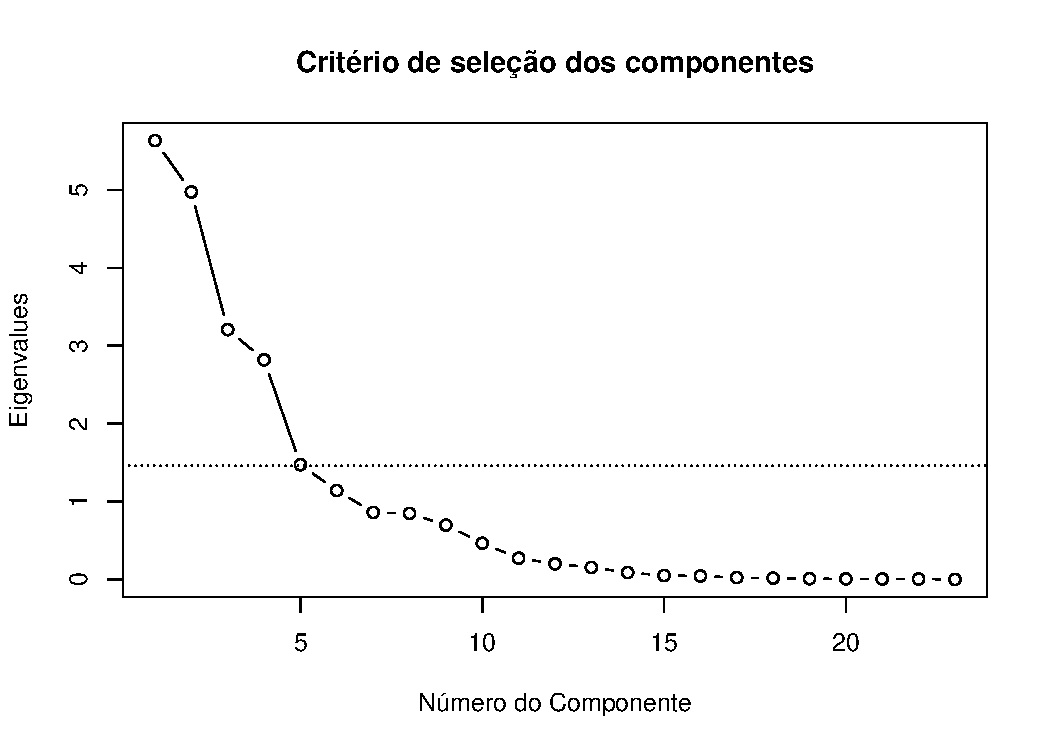
\includegraphics[scale=.80]{../../graficos/latex-graph-scree-plot-pca.pdf}
		\caption{Critério de seleção dos componentes: a partir do 5º componente, observa-se redução no decaimento da variabilidade, o que diminui a importância do componente para uma possível seleção.}
		\label{fig: scree-plot-pca}
\end{figure}

\subsubsection{Características dos Componentes}
A tabela \ref{tbl:caracteristicas-dos-componentes} apresenta com mais clareza os pesos atribuídos aos 4 primeiros componentes pela aplicação da ACP.

% Please add the following required packages to your document preamble:
% \usepackage{booktabs}
\begin{table}[H]
\centering
\begin{tabular}{@{}lllll@{}}
\toprule
\textbf{} & \textbf{PC1} & \textbf{PC2} & \textbf{PC3} & \textbf{PC4} \\ \midrule
CI        & -0.0849      & 0.1032       & 0.6388       & 0.7223       \\
CP        & -0.0748      & 0.1076       & 0.6423       & 0.7344       \\
NBFG      & 0.1748       & 0.6244       & -0.2712      & 0.2344       \\
NBCE      & 0.2362       & 0.6789       & -0.4401      & 0.1951       \\
NBG       & 0.2452       & 0.732        & -0.4448      & 0.2226       \\
NCE       & 0.2849       & 0.7246       & -0.4295      & 0.2552       \\
NBODP     & 0.8914       & -0.3083      & 0.0949       & -0.0112      \\
NPODP     & 0.8906       & -0.327       & 0.1124       & -0.0083      \\
NBIIF     & 0.9189       & -0.2369      & 0.1209       & -0.017       \\
NPIIF     & 0.9185       & -0.2368      & 0.1453       & -0.0077      \\
NBOAF     & 0.9175       & -0.1637      & 0.1402       & -0.033       \\
NPOAF     & 0.9124       & -0.1723      & 0.1478       & -0.03        \\
CPNE      & -0.0899      & 0.1519       & 0.6207       & 0.7365       \\
PCPNE     & -0.0035      & 0.1788       & -0.124       & 0.0935       \\
NBIDD     & 0.4134       & 0.3794       & -0.4194      & 0.3308       \\
NPIDD     & 0.439        & 0.3988       & -0.4431      & 0.3344       \\
ND        & -0.0428      & 0.3428       & 0.2322       & 0.2084       \\
NBM       & 0.1568       & 0.6534       & 0.3918       & -0.3426      \\
NPM       & 0.1542       & 0.6309       & 0.4099       & -0.3402      \\
NBD       & 0.0692       & 0.6702       & 0.3762       & -0.3727      \\
NPD       & 0.0741       & 0.6629       & 0.3857       & -0.3727      \\
NBRT      & 0.0739       & 0.4969       & 0.3134       & -0.334       \\
NPRT      & 0.0727       & 0.4829       & 0.3175       & -0.332       \\ \bottomrule
\end{tabular}
\caption{Características dos Componentes}
\label{tbl:caracteristicas-dos-componentes}
\end{table}

De acordo com \citeonline[p.~107]{larose2015data} o peso dos componentes representa a relação do mesmo com a variável. Para que o peso de um componente tenha significância prática este deve exceder $\pm.50$ em magnitude. Desta forma, a tabela \ref{tbl:caracteristicas-dos-componentes} apresenta a mesma informação, sendo omitidos os pesos menores que 0.5.

% Please add the following required packages to your document preamble:
% \usepackage{booktabs}
\begin{table}[H]
\centering
\begin{tabular}{@{}lllll@{}}
\toprule
\textbf{} & \textbf{PC1} & \textbf{PC2} & \textbf{PC3} & \textbf{PC4} \\ \midrule
CI        &              &              & 0.6388       & 0.7223       \\
CP        &              &              & 0.6423       & 0.7344       \\
NBFG      &              & 0.6244       &              &              \\
NBCE      &              & 0.6789       &              &              \\
NBG       &              & 0.732        &              &              \\
NCE       &              & 0.7246       &              &              \\
NBODP     & 0.8914       &              &              &              \\
NPODP     & 0.8906       &              &              &              \\
NBIIF     & 0.9189       &              &              &              \\
NPIIF     & 0.9185       &              &              &              \\
NBOAF     & 0.9175       &              &              &              \\
NPOAF     & 0.9124       &              &              &              \\
CPNE      &              &              & 0.6207       & 0.7365       \\
PCPNE     &              &              &              &              \\
NBIDD     &              &              &              &              \\
NPIDD     &              &              &              &              \\
ND        &              &              &              &              \\
NBM       &              & 0.6534       &              &              \\
NPM       &              & 0.6309       &              &              \\
NBD       &              & 0.6702       &              &              \\
NPD       &              & 0.6629       &              &              \\
NBRT      &              &              &              &              \\
NPRT      &              &              &              &              \\ \bottomrule
\end{tabular}
\caption{Componentes com magnitudes $\pm.50$}
\label{my-label}
\end{table}

Determinados os pesos, é possível agora classificar os componentes principais de acordo com sua estrutura e pesos nas variáveis:

\begin{enumerate}
\item O primeiro componente (PC1) apresenta pesos significativos nas variáveis  \textit{Organização Didático-pedagógica}, \textit{Infra-estrutura e Instalações} e \textit{Oportunidades de Ampliação da Formação}. Com base nisto é possível concluir que esse componente apresenta um perfil do que o curso é capaz de entregar ao aluno, que é refletida nas notas que o mesmo atribui no momento da avaliação.
\item Em PC2 observamos uma concentração dos pesos nas variáveis associadas a duas dimensões: alunos e professores. No que se refere aos alunos, pesam mais as notas avaliadas de acordo com o desempenho dos mesmos nas provas nas áreas de \textit{Formação Geral} e \textit{Conhecimentos Específicos}. Já em relação aos professores tem destaque as variáveis \textit{Quantidade de Mestres} e \textit{Quantidade de Doutores} nos cursos.
\item Em PC3 têm destaque as variáveis \textit{Concluíntes Inscritos} e \textit{Percentual de Concluíntes Participantes com nota no Enem}. Isso indica que este componente tem um perfil mais voltado a determinar a situação dos alunos no censo bem como a contabilização da participação dos mesmos.
\item PC4 apresenta perfil de composição similar à PC3. Os pesos, por sua vez, apresentam magnitudes levemente superiores. Isso se deve ao fato de esse componente ter tido uma proporção de variância individual menor em relação a PC3 (13,9\% contra 21,6\%) como pode ser observado na listagem \ref{lst:loadings_pca}. Desta forma, apesar de este componente ter apresentado pesos relativamente maiores, sua variância total menor faz com que seja posicionado em 4º na ordem dos componentes.
\end{enumerate}

%Enviado para a sessão Resultados, após comentário no Schoology em 10/7 às 9:39 am.
%Por meio da aplicação da análise do componente principal foi possível identificar características relevantes sobre as variáveis preditoras do CPC. A referida análise também possibilitou o agrupamento destas variáveis em componentes principais. Verificou-se que o primeiro (principal) componente apresenta afinidade com o que o curso e a instituição de ensino dipõem em termos de profissionais (Organização Didático-pedagógica), estrutura (Infra-estrutura e Instalações) e perspectiva do futuro, do ponto de vista do aluno (Oportunidades de Ampliação da Formação). A pontuação nestas variáveis tem origem em avaliação subjetiva do aluno participante do censo. A classificação destas variáveis como constantes no primeiro componente permite-nos afirmar que um maior desempenho nestes quesitos implicará em maior resposta na variável dependente (CPC Contínuo).

%!TEX root = ../main/main.tex
\subsection{Análise do Fator}

A análise do componente principal apresentou quais variáveis são passíveis de melhor explicarem o que influencia no desempenho do curso no CPC. Foi apresentado o conjunto de variáveis e o perfil de cada componente. Contudo, é oportuno incluir mais uma camada de robustez à pesquisa pela aplicação da Análise do Fator -- AF ou (\textit{Factor Analysis} -- FA). \citeonline[p.~110--111]{larose2015data} destaca que, apesar de a ACP e AF serem técnicas de análise multivariada bem similares, a ACP deve ser em essência, um meio para a consecução da AF. 

De acordo com \citeonline[p.~93]{hair1998multivariate} a AF desempenha um papel importante na identificação das interações entre as variáveis por intermédio do agrupamento (em fatores) das mesmas de acordo com seu grau de relação. Esse procedimento permite a redução da dimensionalidade. Isso quer dizer que procura-se descrever um evento utilizando um conjunto menor de variáveis relativamente ao conjunto original estudado com o mínimo de perda de informação.

Vale ressaltar que as conclusões desta pesquisa tem perspectiva exploratória. Procura-se por meio do AF estabelecer uma estrutura nos dados do Enade utilizando este método como técnica de redução. Essa abordagem é diferente da confirmatória pois não são utilizados testes para se chegar a uma estrutura esperada com base em hipóteses. \Ibidem{hair1998multivariate}.

De acordo com \citeonline[p.~111]{larose2015data}, precedem a aplicação da AF os seguintes procedimentos: (i) padronização das variáveis; (ii) determinação dos vetores-Z (ou \textit{Z-vectors}) e (iii) a matriz de correlação.

Na figura \ref{fig: matriz-correlograma} vemos a reapresentação da matriz de correlação das variáveis preditoras agrupadas em \textit{clusters} de acordo com a intensidade de correlação. 

\begin{figure}[H]
		\centering
		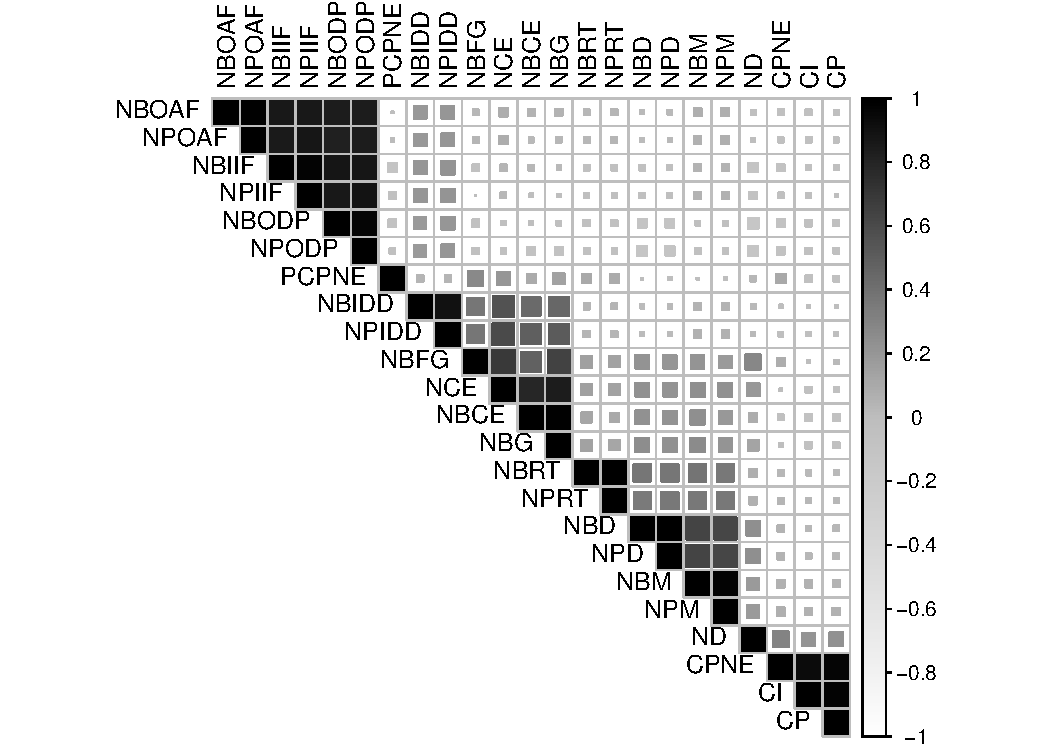
\includegraphics[scale=.75]{../../graficos/latex-graph-matriz-correlacao}
		\caption{Matriz correlograma}
		\label{fig: matriz-correlograma}
\end{figure}

Para que seja empregada de forma correta, a AF requer que as variáveis estejam minimamente correlacionadas. Neste sentido, \citeonline[p.~112]{larose2015data} recomendam a realização do teste de \textit{Esfericidade de Bartlett} para determinar se existe um nível mínimo de correlação como fase preliminar à aplicação da AF. Seguindo este autor, o referido teste foi realizado nos dados padronizados das variáveis do \textit{dataset} em questão. O resultado é apresentado na listagem \ref{lst:teste_de_bartlett}.
\pagebreak
\begin{lstlisting}[label={lst:teste_de_bartlett}, caption={Teste de Esfericidade de Bartlett}, captionpos=b]
$chisq
[1] 469552.9
$p.value
[1] 0
$df
[1] 300
\end{lstlisting}

O teste de Bartlett verifica a \textit{hipótese nula} de que a matriz de correlação é uma matriz identidade, sendo as variáveis portanto não correlacionadas. A principal informação deste teste é o valor de p (ou \textit{p-value}). Valores muito acima de 0.10 indicam que a aplicação do AF pode não ser adequada. Por outro, lado valores pequenos indicam que há evidências contra a hipótese nula, consequentemente validando o método. Como observado na saída acima, o \textit{p-value} é 0 o que indica que o AF pode ser aplicada.

Na listagem \ref{lst:loadings_fa_antes_rotacao} são apresentados os dois resultados da aplicação da função \lstinline{fa} sobre os dados padronizados. O primeiro resultado contém os \textit{eigenvalues} de cada variável preditora computada. O segundo contém os carregamentos (ou \textit{loadings}) juntamente à proporção de variância e variância acumulada.

\begin{lstlisting}[label={lst:loadings_fa_antes_rotacao}, captionpos=b, 
caption={Carregamentos da AF: o primeiro fator demonstra similaridade com o primeiro componente da ACP o que confirma a solidez e consistência das constatações até aqui verificadas.}]
 [1]  6.82829446  5.06102146  3.02305954  2.57594785  0.89229036  0.73263127  0.44322564  0.32873650  0.12874448
[10]  0.09205939  0.02032373 -0.01542126 -0.02141875 -0.04602155 -0.05979722 -0.08471119 -0.09794112 -0.11387848
[19] -0.13637542 -0.23237097 -0.27069873 -0.29403878 -0.29933457 -0.31091515 -0.65475511

Loadings:
      PA1    PA2    PA3    PA4   
CI            0.129  0.844  0.451
CP            0.128  0.866  0.470
NBFG   0.453  0.382 -0.135  0.247
NBCE   0.552  0.415 -0.294  0.297
NBG    0.596  0.461 -0.299  0.332
NCE    0.652  0.446 -0.285  0.365
NBODP  0.551 -0.753              
NPODP  0.545 -0.772  0.100       
NBIIF  0.613 -0.713  0.110       
NPIIF  0.614 -0.715  0.135       
NBOAF  0.641 -0.650  0.122       
NPOAF  0.633 -0.654  0.129       
CPNE          0.172  0.835  0.469
PCPNE         0.123              
NBIDD  0.583  0.103 -0.241  0.406
NPIDD  0.628  0.108 -0.267  0.431
ND     0.125  0.258  0.222       
NBM    0.462  0.423  0.264 -0.463
NPM    0.452  0.407  0.278 -0.463
NBD    0.420  0.493  0.242 -0.495
NPD    0.422  0.486  0.250 -0.498
NBRT   0.307  0.322  0.167 -0.342
NPRT   0.300  0.312  0.170 -0.340
CPCC   0.958  0.248              
CPCF   0.862  0.219              

                 PA1   PA2   PA3   PA4
SS loadings    6.828 5.061 3.023 2.576
Proportion Var 0.273 0.202 0.121 0.103
Cumulative Var 0.273 0.476 0.596 0.700
\end{lstlisting}

Observa-se que os quatro primeiros fatores computam uma variância de 68,4\% -- ligeiramente menor quando comparado à variância acumulada da mesma quantidade de componentes principais na fase de aplicação da ACP que foi de 72,3\%. É verificado também que, assim como na ACP, o primeiro fator é o que possui a maior variância.

Quanto a seleção de fatores, o mesmo critério foi utilizado em relação à escolha dos componentes na ACP: \textit{Scree plot} \cite[p.~109]{hair1998multivariate}. O gráfico da figura \ref{fig: fa-scree-plot} demonstra que a partir do 5º fator há uma tendência à estabilização em relação à variância explicada pelos fatores individuais.

\begin{figure}[H]
		\centering
		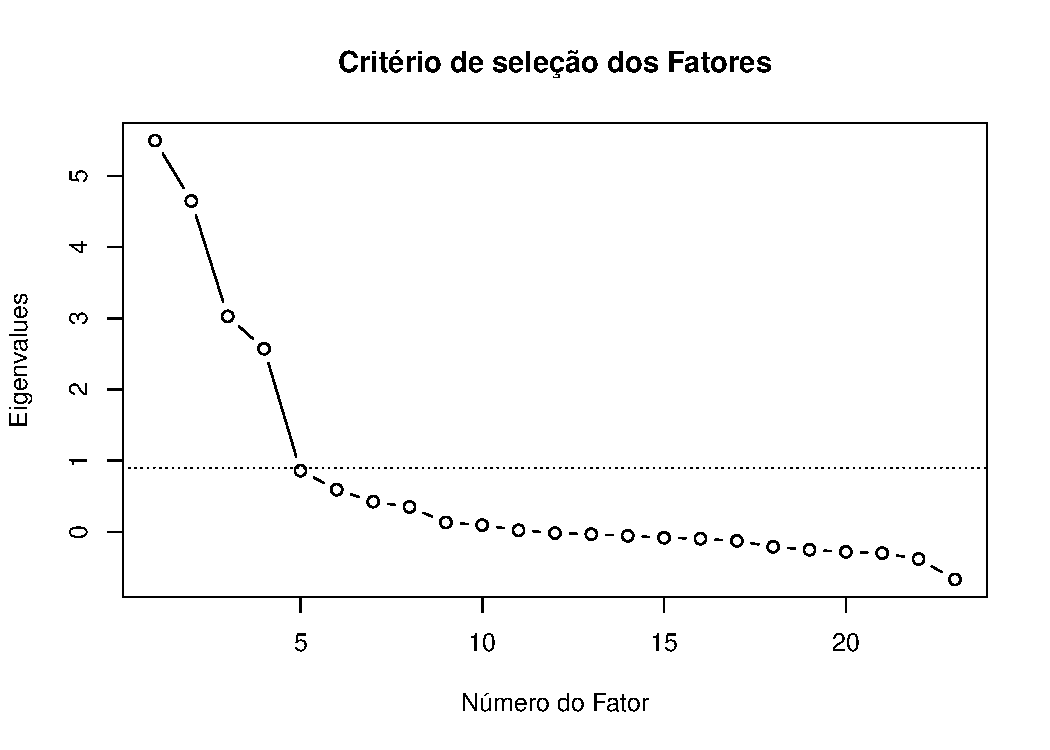
\includegraphics[scale=.75]{../../graficos/latex-graph-fa-scree-plot.pdf}
		\caption{Critério de seleção dos fatores: a partir do 5º fator, observa-se uma tendência de horizontalização da curva de variabilidade explicada pelos fatores, o que torna os fatores a partir desta contagem menos suscetíveis em participar de uma seleção.}
		\label{fig: fa-scree-plot}
\end{figure}

\subsubsection{Rotação dos Fatores}

A rotação dos fatores consiste em um elemento de validação da Análise do Fator. De acordo com \citeonline[p.~112]{hair1998multivariate}, a rotação serve para redistribuir as proporções de variância residuais dos fatores mais afastados para os iniciais. \citeonline[p.~114]{larose2015data} faz a analogia de um cientista tentando obter maior resolução em uma imagem ao ajustar o foco de seu microscópio.

\begin{lstlisting}[label={lst:loadings_fa_apos_rotacao}, caption={Carregamentos da AF após rotação}, captionpos=b]
Loadings:
      PA2    PA1    PA4    PA3   
CI                          0.965
CP                          0.993
NBFG          0.627  0.176       
NBCE          0.791  0.151       
NBG           0.857  0.168       
NCE           0.900  0.168       
NBODP  0.934                     
NPODP  0.947                     
NBIIF  0.947                     
NPIIF  0.953                     
NBOAF  0.919                     
NPOAF  0.918                     
CPNE                        0.972
PCPNE         0.169              
NBIDD  0.215  0.725              
NPIDD  0.233  0.779              
ND            0.133  0.212  0.255
NBM           0.122  0.811       
NPM           0.104  0.804       
NBD           0.114  0.841       
NPD           0.108  0.843       
NBRT                 0.580       
NPRT                 0.571       
CPCC   0.395  0.741  0.524       
CPCF   0.358  0.667  0.468       

                 PA2   PA1   PA4   PA3
SS loadings    5.672 4.814 4.056 2.946
Proportion Var 0.227 0.193 0.162 0.118
Cumulative Var 0.227 0.419 0.582 0.700

\end{lstlisting}

A rotação de fatores pode ser entendida como o esforço para obtenção da melhor configuração de variâncias no plano cartesiano. A listagem \ref{lst:loadings_fa_apos_rotacao} demonstra a rotação pelo método \textit{Varimax} que maximiza a variabilidade para cada coluna. Pela comparação com a listagem \ref{lst:loadings_fa_antes_rotacao}, percebe-se que variabilidades maiores são obtidas após a rotação.

%\subsubsection{Considerações sobre os Fatores}

%Enviado para a sessão Resultados, após comentário no Schoology em 10/7 às 9:39 am.
%É possível verificar grande semelhança nos resultados das análises multivariadas AF e ACP no que se refere à composição do conjunto de variáveis que representam a redução de dimensionalidade. Por esse motivo, entende-se o caráter corroborativo da AF em relação ao ACP nesta pesquisa. Em termos de perfis de variáveis para cada fator, os mesmos não diferem dos perfis elaborados para ACP.

\pagebreak